

\chapter{Rotational Kinematics}
\begin{marginfigure}%
  \includegraphics[width=\linewidth]{nerd5.jpg}
  \caption{Turntablism is largely an art of rotational kinematics}
  \label{fig:marginfig}
\end{marginfigure}
\textit{Joy is the mainspring... in Nature's calm rotation.}  \\
\noindent\textbf{-Friedrich Schiller}
\vspace{1cm}
\section{Pure Rotation}

\begin{margintable}[50pt]
\begin{center}
\footnotesize
\begin{tabular}{lllll}
\toprule
 Translation         & Rotation                                                    \\
\midrule
  Position $(x)$  & Angle $(\theta)$       \\
  Velocity $(v)$ & Angular Velocity$(\omega)$           \\
   Acceleration $(a)$  & Angular Acceleration$(\alpha)$                        \\
\bottomrule
\end{tabular}
\end{center}
  \caption{Translational and rotational analogues}
  \label{tab:font-sizes}
\end{margintable}

$$
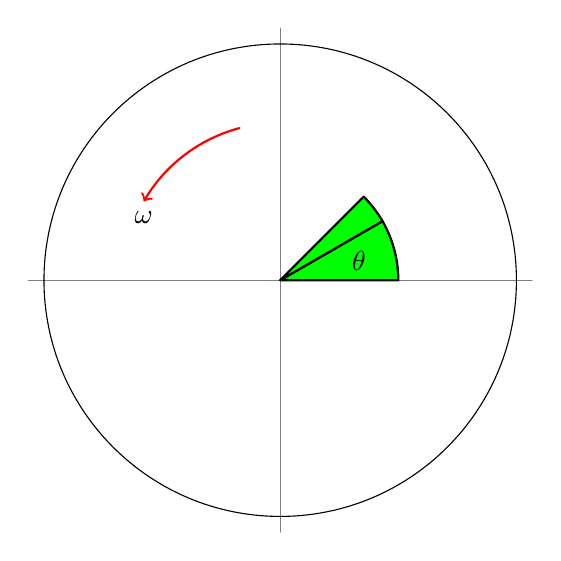
\begin{tikzpicture}
    [line cap=round,line join=round,x=2cm,y=2cm, scale=1, decoration={brace,amplitude=2pt}]


%\draw[->, xshift=0cm]  (120:2.4cm) arc (120:170:2.4) node[below] {$\omega$};
    \draw[color=gray,thin] (-1.6,0) -- (1.6,0)  ;
   \draw[color=gray,thin] (0,-1.6) -- (0,1.6);
  
 
  \draw[thick,red,->] ([shift=(105:2cm)]0,0) arc (105:150:2cm) node [below, black] {$\omega$};
  \draw (0,0) circle (3cm);
  \draw[fill=green, thick ] ([shift=(0:1.5cm)]0,0) arc (0:30:1.5cm) -- (0,0) -- cycle;
   \draw[fill=green, thick ] ([shift=(30:1.5cm)]0,0) arc (30:45:1.5cm) -- (0,0) -- cycle;
   \draw (0.5,0) node [anchor=south ,scale=1] {$\theta$};
  
    %  \fill[black] (0,0.1) circle (0.3mm) node [anchor=south east,scale=1] {\scriptsize$ \theta(0)$};

    % \draw (0.6,0.8) node [anchor=south west ,scale=1] {$\theta(t)$};
    
 \end{tikzpicture}
$$

\subsubsection{Angular Velocity}
\marginnote[0pt]{The angular velocity is the rate of change of the angle value.  The lowercase Greek letter omega is used to represent it as an algebraic variable.}
$$\omega=\lim_{\Delta \rightarrow 0}\frac{\Delta \theta}{\Delta t}$$
$$\bar{\omega}=\frac{\Delta \theta}{\Delta t}=\frac{2\pi \theta}{T}$$

\subsubsection{Angular Acceleration}
\marginnote[0pt]{Angular acceleration is the time rate of change of the angular velocity.  The lowercase Greek letter alpha is used to represent it as an algebraic variable.}
$$\alpha=\lim_{\Delta \rightarrow 0}\frac{\Delta \omega}{\Delta t}$$

\subsection{Kinematics Equations for Angular Motion}


\subsubsection{Constant Angular Velocity}
\marginnote[0pt]{Under zero acceleration the angular velocity is constant.  The angle is a linear function of time with a slope equal to the angular velocity.}
$$\alpha=0$$
$$\omega=\omega_0$$
$$\theta=\theta_0+\omega t$$

\subsubsection{Constant Angular Acceleration}
\marginnote[0pt]{Under constant acceleration the angular velocity is a linear function of time with a slope equal to the angular acceleration.  The angle is a quadratic function of time.  The angular velocity may also be parameterized as a function of angle.}
$$\omega=\omega_0+\alpha t$$
$$\bar{\omega}=\frac{\omega_0+\omega}{2}$$
$$\theta=\theta_0+\omega_0t+\frac{\alpha t^2}{2}=\theta_0+\bar{\omega}t$$
$$\omega^2-\omega_0^2=2\alpha(\theta-\theta_0)$$


\subsubsection{Variable Angular Acceleration}
\marginnote[70pt]{$$\Delta \omega=\text{Area under }\alpha(t)$$ }
$$
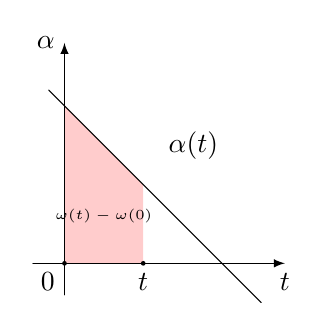
\begin{tikzpicture}
    [line cap=round,line join=round,x=2cm,y=2cm, scale=1, decoration={brace,amplitude=2pt}]

\fill[fill=red!20] (0,0) -- plot [domain=0:.5] (\x,{1-\x}) -- plot [domain=0.5: 0.0] (\x,0) -- cycle;

 \draw[smooth,samples=100,domain=-0.1:1.25]
                                 plot(\x,{1-\x});

    \fill[black] (0,0) circle (0.3mm) node [anchor=north east,scale=1] {$ 0$};
     \fill[black] (0.5,0) circle (0.3mm) node [anchor=north ,scale=1] {$t$};

  \draw[-latex,color=black,thin] (-0.2,0) -- (1.4,0) node [anchor=north ,scale=1] {$t$};
   \draw[-latex,color=black,thin] (0,-0.2) -- (0,1.4)node [anchor=east ,scale=1] {$\alpha$};
    \draw (0.6,0.6) node [anchor=south west ,scale=1] {$\alpha(t)$};
        \draw (0.25,0.3) node [anchor=center ,scale=1] {\tiny$\omega(t)-\omega(0)$};
        
 \end{tikzpicture}
$$
\marginnote[70pt]{$$\omega(t)=\omega(0)+\text{Area}(\alpha(t))$$
$$\Delta \theta=\text{Area under }\omega(t)$$ }
$$
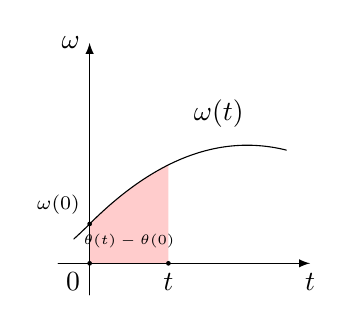
\begin{tikzpicture}
    [line cap=round,line join=round,x=2cm,y=2cm, scale=1, decoration={brace,amplitude=2pt}]

\fill[fill=red!20] (0,0) -- plot [domain=0:.5] (\x,{-\x^2/2+\x+0.25}) -- plot [domain=0.5: 0.0] (\x,0) -- cycle;

 \draw[smooth,samples=100,domain=-0.1:1.25]
                                 plot(\x,{-\x^2/2+\x+0.25});

    \fill[black] (0,0) circle (0.3mm) node [anchor=north east,scale=1] {$ 0$};
     \fill[black] (0.5,0) circle (0.3mm) node [anchor=north ,scale=1] {$t$};
      \fill[black] (0,0.25) circle (0.3mm) node [anchor=south east,scale=1] {\scriptsize$ \omega(0)$};

  \draw[-latex,color=black,thin] (-0.2,0) -- (1.4,0) node [anchor=north ,scale=1] {$t$};
   \draw[-latex,color=black,thin] (0,-0.2) -- (0,1.4)node [anchor=east ,scale=1] {$\omega$};
     \draw (0.6,0.8) node [anchor=south west ,scale=1] {$\omega(t)$};
        \draw (0.25,0.25) node [anchor=north ,scale=1] {\tiny$\theta(t)-\theta(0)$};
        
 \end{tikzpicture}
$$
\marginnote[70pt]{$$\theta(t)=\theta(0)+\text{Area}(\omega(t))$$ }
$$
\begin{tikzpicture}
    [line cap=round,line join=round,x=2cm,y=2cm, scale=1, decoration={brace,amplitude=2pt}]


 \draw[smooth,samples=100,domain=-0.1:1.25]
                                 plot(\x,{-\x^3/6+\x^2/2+\x/4+0.1});
  
      \fill[black] (0,0.1) circle (0.3mm) node [anchor=south east,scale=1] {\scriptsize$ \theta(0)$};
  \draw[-latex,color=black,thin] (-0.2,0) -- (1.4,0) node [anchor=north ,scale=1] {$t$};
   \draw[-latex,color=black,thin] (0,-0.2) -- (0,1.4)node [anchor=east ,scale=1] {$x$};
     \draw (0.6,0.8) node [anchor=south west ,scale=1] {$\theta(t)$};
    
 \end{tikzpicture}
$$

\newpage
\section{Angular and Radial Motion in Polar Coordinates}
\begin{figure}
$$
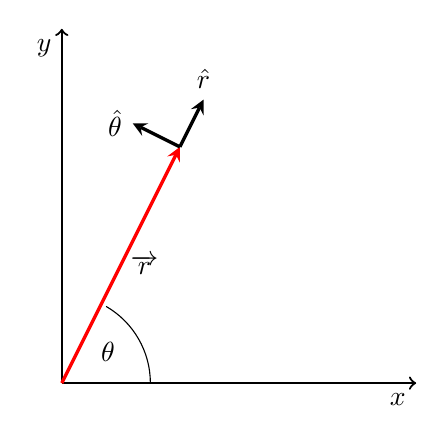
\begin{tikzpicture}[scale=1.5]


\draw[thick,->] (0,0,0) -- (3,0,0) node[anchor=north east]{$x$};
\draw[thick,->] (0,0,0) -- (0,3,0) node[anchor=north east]{$y$};


%draw a vector from origin to point (P) 
\draw[-stealth,very thick,color=red] (0,0) -- (1,2) node[anchor=south west,color=black]{$ $};
\draw[color=red] (0,0) -- (0.5,1) node[anchor=west ,color=black]{$\overrightarrow{r}$};
\draw[-stealth,very thick,color=black] (1,2) -- (1.2,2.4) node[anchor=south,color=black]{$\hat{r}$};
\draw[-stealth,very thick,color=black] (1,2) -- (0.6,2.2) node[anchor=east,color=black]{$\hat{\theta}$};


%draw projection on xy plane, and a connecting line
\draw (0.75,0) arc (0:60:0.75) ;
\draw (0.25,0.1) node [anchor=south west,color=black]{$\theta$};



\end{tikzpicture}
$$
 \caption{Position of a particle in polar coordintes}
  \label{fig:marginfig}
\end{figure}

\newthought{The unit vector in the radial direction} is determined by normalizing the position vector.  This is done by dividing the position vector by its magnitude.  
$$\hat{r}=\frac{\overrightarrow{r}}{r}=\frac{x\hat{x}+y\hat{y}}{\sqrt{x^2+y^2}}=\frac{r\cos \theta\hat{x}+r\sin \theta\hat{y}}{\sqrt{(r\cos \theta)^2+(r\sin \theta)^2}}=\cos \theta\hat{x}+\sin \theta\hat{y}=\left(\begin{array}{c} \cos \theta\\  \sin \theta\end{array}\right)$$
\noindent Perpendicular to the radial unit vector is the unit angular vector.  It points in the direction of increasing angle.

$$\hat{\theta}=-\sin \theta \hat{x}+\cos \theta\hat{y}=\left(\begin{array}{c}-\sin \theta\\  \cos \theta\end{array}\right)$$

\noindent The two unit vectors are orthogonal and together provide a handy coordinate system well suited for rotating systems.
$$\hat{r}\cdot{\hat{\theta}}=0$$

\subsection{Arc Length}
\marginnote[0pt]{For a fixed radius the arc length of a curve is the product of the radius and the angular change.  Angle is measured in radians.}
$$\Delta S= r \Delta \theta$$

\vspace{1cm}

\subsection{Period}
\marginnote[0pt]{The characteristic time for one whole rotation to occur is called the period.}
$$\text{time for a complete rotation}=T$$

\newpage
\subsection{Velocity}

\vspace{1cm}

\marginnote[0pt]{This figure shows change in position expressed in terms of polar components, in the radial direction and the angular (tangential) direction.}

\begin{center}
\begin{tabular}{cc}
\begin{minipage}{7cm}
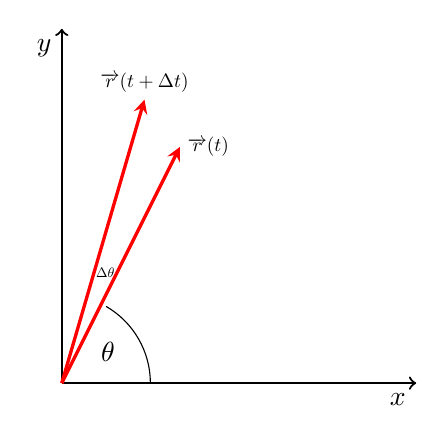
\begin{tikzpicture}[scale=1.5]


\draw[thick,->] (0,0,0) -- (3,0,0) node[anchor=north east]{$x$};
\draw[thick,->] (0,0,0) -- (0,3,0) node[anchor=north east]{$y$};


%draw a vector from origin to point (P) 
\draw[-stealth,very thick,color=red] (0,0) -- (1,2) node[anchor=west,color=black, scale=0.7]{$\overrightarrow{r}(t) $};
\draw[-stealth,very thick,color=red] (0,0) -- (0.7,2.4)node[anchor=south,color=black, scale=0.7]{$\overrightarrow{r}(t+\Delta t) $};
%\draw[color=red] (0,0) -- (0.5,1) node[anchor=west ,color=black]{$\overrightarrow{r}(t)$};



%draw projection on xy plane, and a connecting line
\draw (0.75,0) arc (0:60:0.75) ;
\draw (0.25,0.1) node [anchor=south west,color=black]{$\theta$};
\draw (0.25,0.85) node [anchor=south west,color=black,scale=0.5]{$\Delta \theta$};
%\draw[-stealth,very thick,color=black] (1,2) -- (0.7,2.4) node[anchor=east,color=black, scale=0.7]{$ $};



\end{tikzpicture}
\end{minipage}
&
\begin{minipage}{7cm}

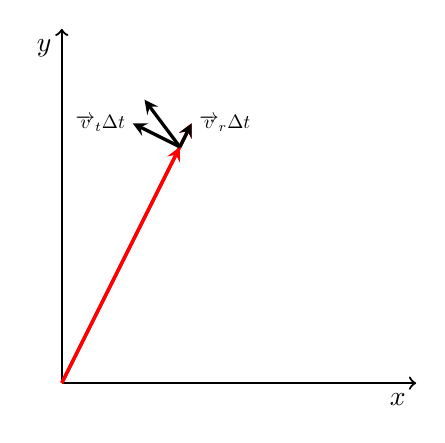
\begin{tikzpicture}[scale=1.5]


\draw[thick,->] (0,0,0) -- (3,0,0) node[anchor=north east]{$x$};
\draw[thick,->] (0,0,0) -- (0,3,0) node[anchor=north east]{$y$};


%draw a vector from origin to point (P) 
\draw[-stealth,very thick,color=red] (0,0) -- (1,2) node[anchor=south west,color=black]{$ $};
\draw[-stealth,very thick,color=red] (0,0) -- (1.1,2.2);
%\draw[color=red] (0,0) -- (0.5,1) node[anchor=west ,color=black]{$\overrightarrow{r}(t)$};
\draw[-stealth,very thick,color=black] (1,2) -- (1.1,2.2) node[anchor=west,color=black, scale=0.7]{$\overrightarrow{v}_r \Delta t$};
\draw[-stealth,very thick,color=black] (1,2) -- (0.6,2.2) node[anchor=east,color=black, scale=0.7]{$\overrightarrow{v}_t \Delta t$};
\draw[-stealth,very thick,color=black] (1,2) -- (0.7,2.4) node[anchor=east,color=black, scale=0.7]{$ $};


%draw projection on xy plane, and a connecting line
%\draw (0.75,0) arc (0:60:0.75) ;
%\draw (0.25,0.1) node [anchor=south west,color=black]{$\theta$};



\end{tikzpicture}



\end{minipage}
\end{tabular}
\end{center}
\vspace{1cm}


\subsubsection{Tangential Velocity}
\marginnote[0pt]{The angular velocity and radius are the two factors contributing to the tangential velocity. }
$$v_{tan}=r\omega$$
$$\overrightarrow{v}_{tan}=v_{tan}\hat{\theta}$$

\subsubsection{Radial Velocity}
\marginnote[0pt]{The radial velocity is the time rate of change of the radius.}
$$v_r=\lim_{\Delta \rightarrow 0}\frac{\Delta r}{\Delta t}$$
$$\overrightarrow{v}_{rad}=v_r\hat{r}$$
\subsubsection{Total Velocity}
\marginnote[0pt]{The total velocity is the vector sum of these two orthogonal components.}
$$\overrightarrow{v}=\lim_{\Delta \rightarrow 0}\frac{\Delta \overrightarrow{r}}{\Delta t}$$
$$\overrightarrow{v}=\underbrace{r\omega\hat{\theta}}_{\textit{tangential}}+\overbrace{v_r\hat{r}}^{\textit{radial}}$$

\vspace{1cm}


\begin{marginfigure}[70pt]%
  \includegraphics[width=\linewidth]{car.jpg}
  \caption{A rad car}
  \label{fig:marginfig}
\end{marginfigure}
\noindent Consider a car driving around a circular racetrack.  The magnitude of the tangential velocity determines how quickly the car circles the track.  The magnitude of the radial velocity determines how quickly the car changes lanes.  

\newpage

\subsection{Acceleration}

\vspace{1cm}

\subsubsection{Tangential Acceleration}
\marginnote[0pt]{The angular acceleration and radius are the two factors contributing to the tangential acceleration. }
$$a_{tan}=r\alpha$$
$$\overrightarrow{a}_{tan}=a_{tan}\hat{\theta}$$
\subsubsection{Centripetal Acceleration}
\marginnote[0pt]{Centripetal acceleration is the acceleration associated with circular motion.   }
$$a_{c}=r\omega^2=\frac{v^2_{tan}}{r}$$
$$\overrightarrow{a}_{c}=-a_{c}\hat{r}$$
\subsubsection{Coriolis Acceleration}
\marginnote[0pt]{The coriolis acceleration is strange.  It is dependent on the velocity in the tangential direction and the radial direction.    }
$$a_{C}=2v_r\omega=\frac{2v_r v_{tan}}{r}$$
$$\overrightarrow{a}_{C}=a_{C}\hat{\theta}$$
\subsubsection{Radial Acceleration}
\marginnote[0pt]{The radial acceleration is simply the time rate of change of the radial velocity.  }
$$a_r=\lim_{\Delta \rightarrow 0}\frac{\Delta v_r}{\Delta t}$$
$$\overrightarrow{a}_{rad}=a_r\hat{r}$$

\subsubsection{Total Acceleration}
\marginnote[0pt]{The total acceleration is the vector sum of these four components.  The centripetal and radial acceleration are in the radial direction.  The coriolis and tangential acceleration are in the tangential direction. }
$$\overrightarrow{a}=\lim_{\Delta \rightarrow 0}\frac{\Delta \overrightarrow{v}}{\Delta t}$$
$$\overrightarrow{a}=\underbrace{r\alpha\hat{\theta}}_{\textit{tangential}}-\overbrace{r\omega^2\hat{r}}^{\textit{centripetal}}+\underbrace{2v_r\omega\hat{\theta}}_{\textit{Coriolis}}+\overbrace{a_r\hat{r}}^{\textit{radial}}$$

\vspace{1cm}

\begin{fullwidth}
\newthought{The Coriolis effect} is a deflection of moving objects when the motion is described relative to a rotating reference frame. In a reference frame with clockwise rotation, the deflection is to the left of the motion of the object; in one with counter-clockwise rotation, the deflection is to the right. Although recognized previously by others, the mathematical expression for the Coriolis force appeared in an 1835 paper by French scientist Gaspard-Gustave Coriolis, in connection with the theory of water wheels.\\ \ \\

Italian scientists Giovanni Battista Riccioli and his assistant Francesco Maria Grimaldi described the effect in connection with artillery in the 1651 Almagestum Novum, writing that rotation of the Earth should cause a cannonball fired to the north to deflect to the east. The effect was described in the tidal equations of Pierre-Simon Laplace in 1778.
\end{fullwidth}

\newpage
\section{Circular Motion}
\marginnote[0pt]{In circular motion the radius is fixed.  There is no radial velocity.    }
\vspace{1cm}
$$v_r=0$$
\marginnote[0pt]{The angular motion may be variable over time with changing speed and acceleration of rotation.  }
$$\{\theta(t),\omega(t), \alpha(t)\}$$
\vspace{1cm}
\marginnote[0pt]{There is only tangental velocity.   }
$$\overrightarrow{v}=\underbrace{r\omega\hat{\theta}}_{\textit{tangential}}+\cancel{\overbrace{v_r\hat{r}}^{\textit{radial}}}=\underbrace{r\omega\hat{\theta}}_{\textit{tangential}}$$
\vspace{1cm}
\marginnote[0pt]{The acceleration has only two terms, the tangential and the centripetal.  The tangential is due to angular acceleration.  The centrifugal is due to the constrained circularity of the motion.}
$$\overrightarrow{a}=\underbrace{r\alpha\hat{\theta}}_{\textit{tangential}}-\overbrace{r\omega^2\hat{r}}^{\textit{centripetal}}+\cancel{\underbrace{2v_r\omega\hat{\theta}}_{\textit{Coriolis}}}+\cancel{\overbrace{a_r\hat{r}}^{\textit{radial}}}=\underbrace{r\alpha\hat{\theta}}_{\textit{tangential}}-\overbrace{r{\omega}^2\hat{r}}^{\textit{centripetal}}=r\alpha\hat{\theta}-\frac{v^2}{r}\hat{r}$$
\vspace{1cm}
\subsection{Circular Motion:  Constant Speed}
\marginnote[0pt]{For circular motion at constant angular velocity the tangential velocity is constant.  There is no angular acceleration therefore and there is no tangential acceleration.  }
\vspace{1cm}
$$\omega(t)=\omega$$
$$\alpha=0$$
$$\theta(t)=\omega t +\theta_0$$
\vspace{1cm}
$$\overrightarrow{v}=r\omega\hat{\theta}=v\hat{\theta}$$
\vspace{1cm}
\marginnote[0pt]{The acceleration is centripetal, towards the center.   }
$$\overrightarrow{a}=\cancel{\underbrace{r\alpha\hat{\theta}}_{\textit{tangential}}}-\overbrace{r{\omega}^2\hat{r}}^{\textit{centrifugal}}=-\frac{v^2}{r}\hat{r}$$

